%\SweaveUTF8




\setkeys{Gin}{width=\textwidth}

\begin{Problem}[Simulation]\label{problem:simulation}
    We continue to use the dataset \code{sepe.dat} (see Problem
    \NR.\ref{problem:characteristics}). We repeatedly draw simple random
    samples without replacement from the $N = 800$ firms.


\begin{Subtask}
    %---------------------------------------------------------------------------
    \item For samples of size $n = 200$, use Monte Carlo simulation to estimate
        the variance of the estimator of mean environmental protection
        expenditures per firm (variable: \code{expend}). Draw 1,000 samples,
        compute the sample mean for each sample, and calculate the variance of
        the 1,000 estimates. Also create a histogram of the estimates.

        Compare the Monte Carlo variance with the theoretical variance from
        Problem \NR.\ref{problem:characteristics}b) and report the coefficient
        of variation of the estimator.

        \begin{Rhint}
            Use \code{replicate(n_sim, expr)}, where \code{n_sim = 1000} and
            \code{expr} draws one sample and computes its sample mean. To
            reproduce the solution, use \code{set.seed(11)} before drawing the
            sample.
        \end{Rhint}

    \begin{Solution}
        We use the dataset \code{sepe.dat}, which contains data for a
        fictitious population of firms:

\begin{Schunk}
\begin{Sinput}
> sepe <- read.table("http://stat.ethz.ch/Teaching/Datasets/WBL/sepe.dat",
                     header = TRUE)
> attach(sepe)
\end{Sinput}
\end{Schunk}

        Let \code{expend} be variable of interest ($y$-variable). Simulate
        1,000 sample means:


\begin{Schunk}
\begin{Sinput}
> n_sim <- 1000
> n <- 200
> N <- 800
> set.seed(11)
> m_mc <- replicate(n_sim, mean(expend[sample(N, n)]))
\end{Sinput}
\end{Schunk}

        The Monte Carlo variance is:

\begin{Schunk}
\begin{Sinput}
> VAR_m_mc <- var(m_mc)
> VAR_m_mc
\end{Sinput}
\begin{Soutput}
[1] 17479711
\end{Soutput}
\end{Schunk}

        Figure \ref{fig:hist_n200} shows the simulated sampling distribution.

\begin{Schunk}
\begin{Sinput}
> hist(m_mc, main = "Histogram of sample means for n = 200")
\end{Sinput}
\end{Schunk}

        \begin{figure}[tbp]
            \centering
            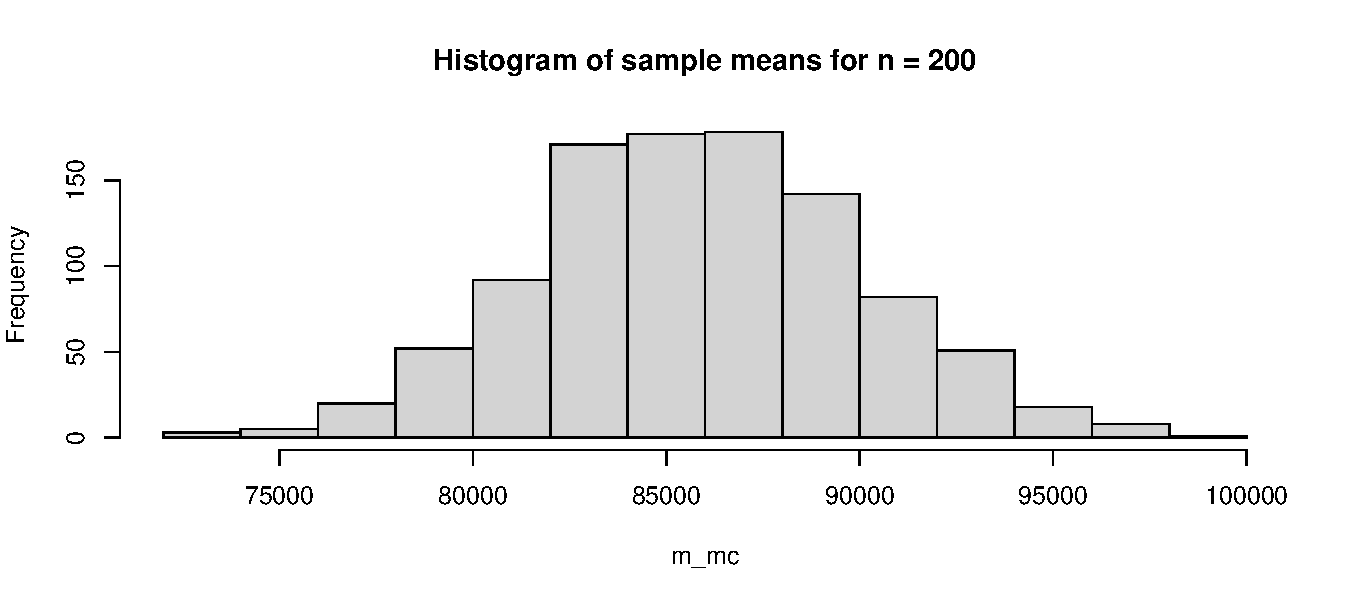
\includegraphics{problems/fig-hist_n200}
            \caption{Simulated sampling distribution ($n = 200$)}
            \label{fig:hist_n200}
        \end{figure}

        Under simple random sampling without replacement,
        \begin{equation*}
            \var(\mys) = \left(1 - \frac{n}{N}\right)\frac{\varyu}{n},
        \end{equation*}
        where
        \begin{equation*}
            \varyu = \frac{1}{N - 1}\sum_{i \in U}(y_i - \myu)^2.
        \end{equation*}
        In R, \code{var(expend)} computes $\varyu$. The theoretical variance is:

\begin{Schunk}
\begin{Sinput}
> VAR_m_y <- (1 - n / N) * var(expend) / n
> VAR_m_y
\end{Sinput}
\begin{Soutput}
[1] 17392015
\end{Soutput}
\end{Schunk}

        The theoretical and Monte Carlo coefficients of variation are:

\begin{Schunk}
\begin{Sinput}
> sqrt(VAR_m_y) / mean(expend)
\end{Sinput}
\begin{Soutput}
[1] 0.04851721
\end{Soutput}
\begin{Sinput}
> sd(m_mc) / mean(m_mc)
\end{Sinput}
\begin{Soutput}
[1] 0.04870305
\end{Soutput}
\end{Schunk}

        The Monte Carlo results are close to the theoretical values.
    \end{Solution}

    %---------------------------------------------------------------------------
    \item Repeat the simulation for samples of size $n = 50$. Compare the
        coefficient of variation with the result from part a).
        Also create a histogram of the estimates.

    \begin{Solution}
        Repeat the simulation with $n = 50$:

\begin{Schunk}
\begin{Sinput}
> n <- 50
> set.seed(11)
> m_mc50 <- replicate(n_sim, mean(expend[sample(N, n)]))
\end{Sinput}
\end{Schunk}

        The Monte Carlo variance is:

\begin{Schunk}
\begin{Sinput}
> VAR_m_mc <- var(m_mc50)
> VAR_m_mc
\end{Sinput}
\begin{Soutput}
[1] 79657236
\end{Soutput}
\end{Schunk}

        Figure \ref{fig:hist_n50} shows the simulated sampling distribution.

\begin{Schunk}
\begin{Sinput}
> layout(matrix(c(1, 2), ncol = 1))
> hist(m_mc, xlim = c(6, 13) * 1E4,
       main = "Histogram of sample means for n = 200")
> hist(m_mc50, xlim = c(6, 13) * 1E4,
       main = "Histogram of sample means for n = 50")
\end{Sinput}
\end{Schunk}

        \begin{figure}[tbp]
            \centering
            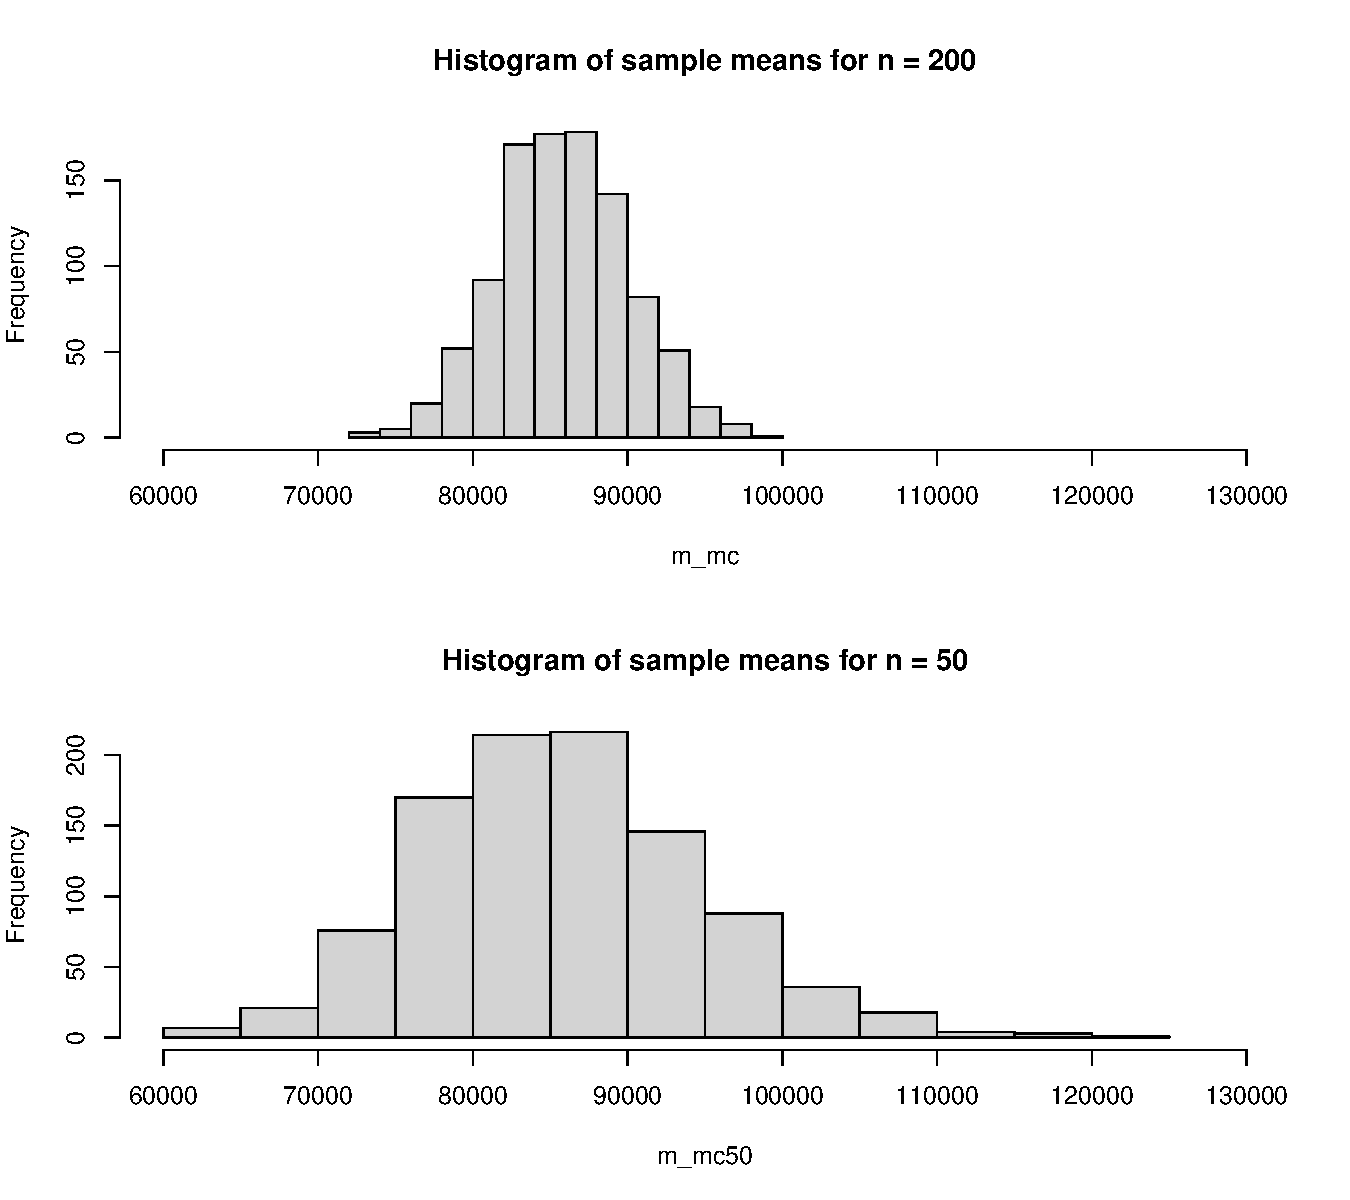
\includegraphics{problems/fig-hist_n50}
            \caption{Simulated sampling distribution ($n = 50$ and $n = 200$;
            x-axis uses the same scale)}
            \label{fig:hist_n50}
        \end{figure}

        The theoretical variance is:

\begin{Schunk}
\begin{Sinput}
> VAR_m_y <- (1 - n / N) * var(expend) / n
> VAR_m_y
\end{Sinput}
\begin{Soutput}
[1] 86960074
\end{Soutput}
\end{Schunk}

        The theoretical and Monte Carlo coefficients of variation are:

\begin{Schunk}
\begin{Sinput}
> sqrt(VAR_m_y) / mean(expend)
\end{Sinput}
\begin{Soutput}
[1] 0.1084878
\end{Soutput}
\begin{Sinput}
> sd(m_mc50) / mean(m_mc50)
\end{Sinput}
\begin{Soutput}
[1] 0.1040796
\end{Soutput}
\end{Schunk}

        With the smaller sample, both the variance and the coefficient of
        variation are larger, as expected.
    \end{Solution}
\end{Subtask}
\end{Problem}
